\chapter{频域分析}

\section{频率特性}

\begin{definition}{频率特性}
    \label{frequency-characteristics}
    我们称$G(j\omega)$为系统（或元件）的频率特性，又称频率响应，可以由系统的传递函数求得：
    \begin{equation*}
        G(j\omega) = G(s)|_{s=j\omega} = \left\lvert G(j\omega) \right\rvert e^{j\phi(\omega)} 
    \end{equation*}

    其中$\phi(\omega) = \angle G(j\omega)$

    频率特性具有以下性质：
    \begin{enumerate}
        \item 频率特性是描述线性定常系统的一种数学模型，只有线性定常系统才有频率特性
        \item 频率特性$G(j\omega)$是一个复变量，它的幅值$\left\lvert G(j\omega) \right\rvert $ 和相角$\phi(\omega)$ 都是频率$\omega$的函数
        \item 系统在频率为$\omega$的正弦输入信号作用下，频率特性反映了输出信号稳态分量和输入信号的关系
        \item 在频率特性中，所用的频率均为角频率$\omega$
        \item 在频率特性中，一般讨论的频率范围是$\omega \in (0,+\infty)$
        \item 频率特性的另一个定义是：频率特性是输出信号Fourier变换式与输入信号Fourier变换式之比
        \item 频率特性是系统脉冲响应的Fourier变换式
    \end{enumerate}
\end{definition}

\subsection{频率特性的几种表示形式}

频率特性$G(j\omega)$是一个复变函数，它是$\omega$的函数。对于连续变化的$\omega$，$G(j\omega)$是复数平面上的一条轨迹

频率特性有以下几种表示形式
\subsubsection{Nyquist图}
将频率特性$G(j\omega)$写成模和幅角的形式，让$\omega$从0变化至$+\infty$，将$G(j\omega)$的轨迹画在复数平面中，即是Nyquist图

典型环节的Nyquist图如下所示：
\begin{center}
    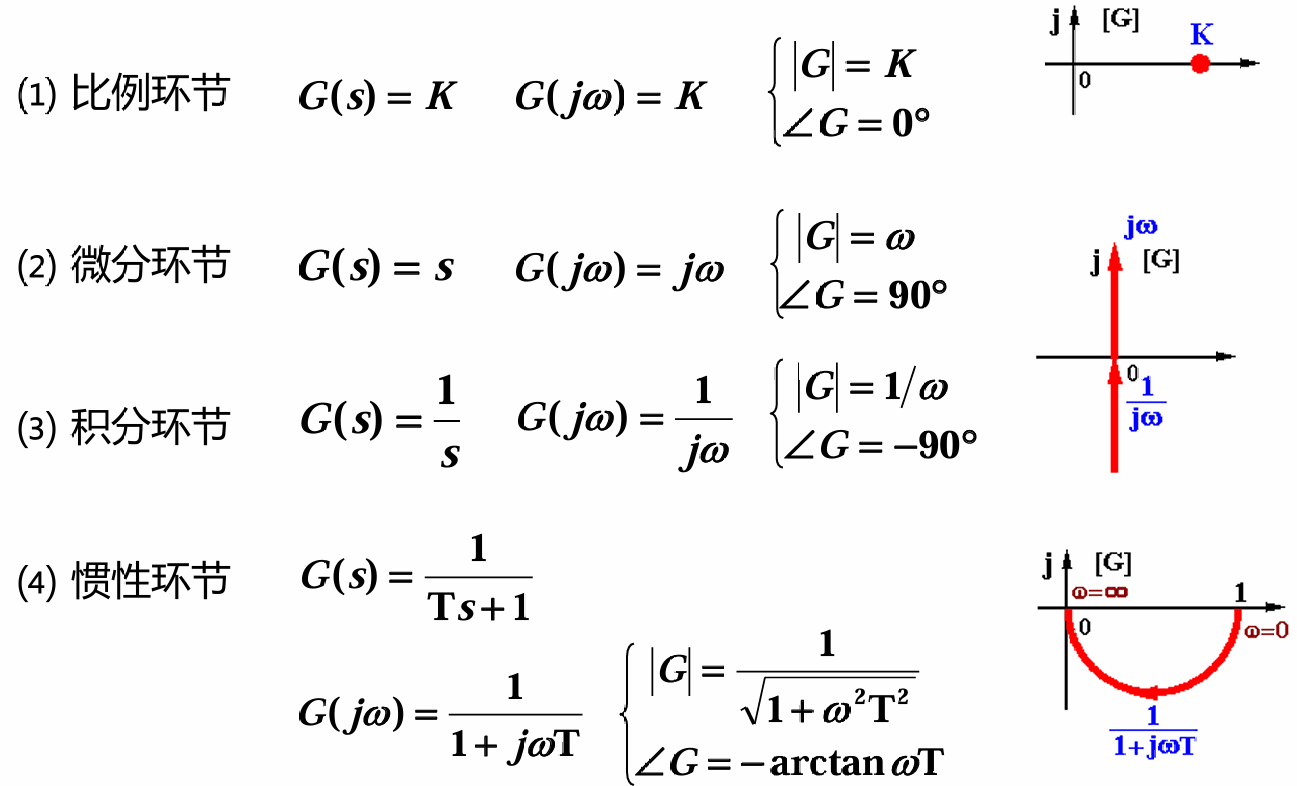
\includegraphics[width=.5\textwidth]{note/frequency-domain analysis/figure/1.png}\\
    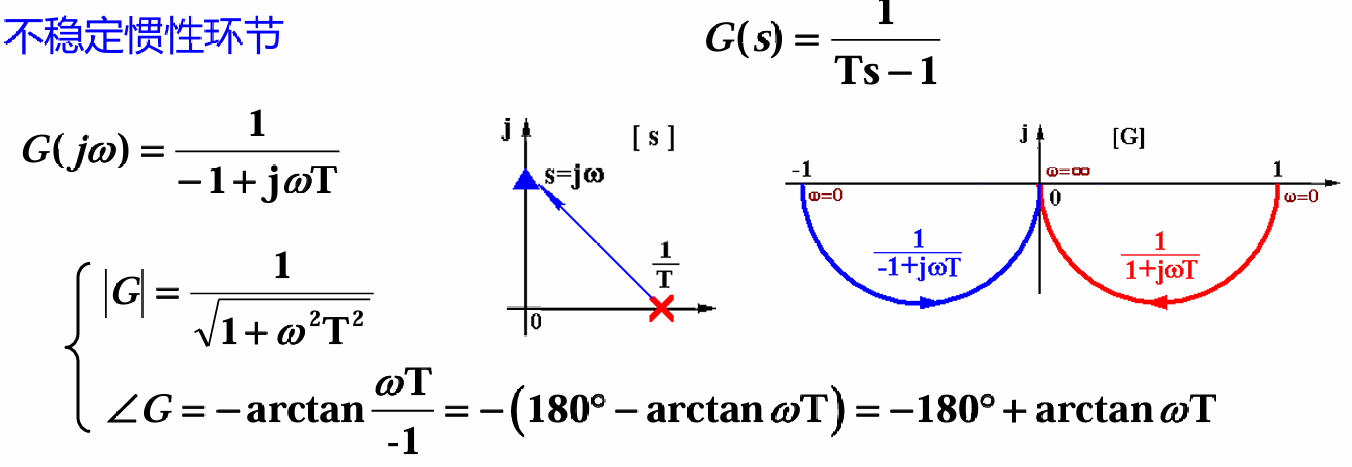
\includegraphics[width=.5\textwidth]{note/frequency-domain analysis/figure/2.png}\\
    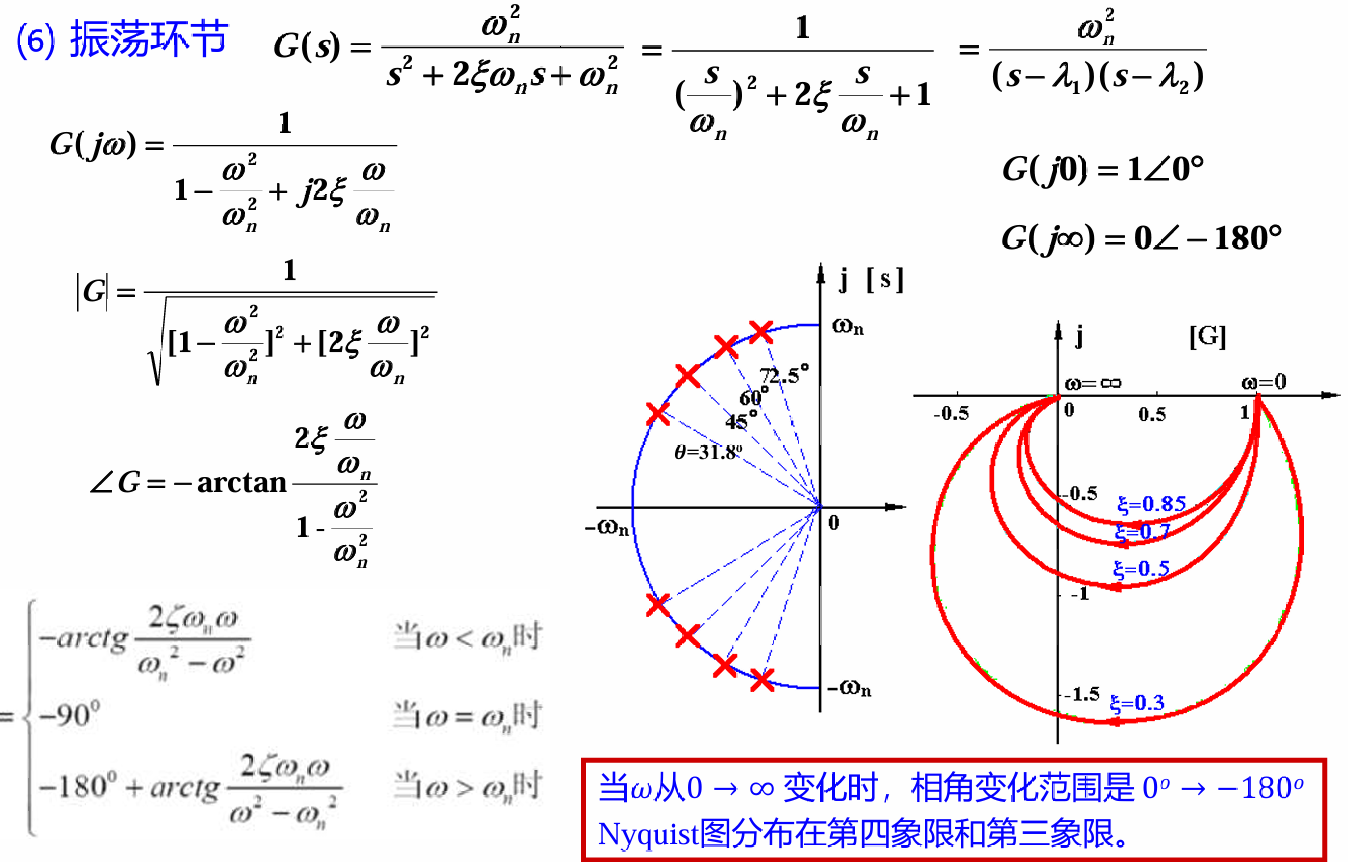
\includegraphics[width=.5\textwidth]{note/frequency-domain analysis/figure/3.png}\\
    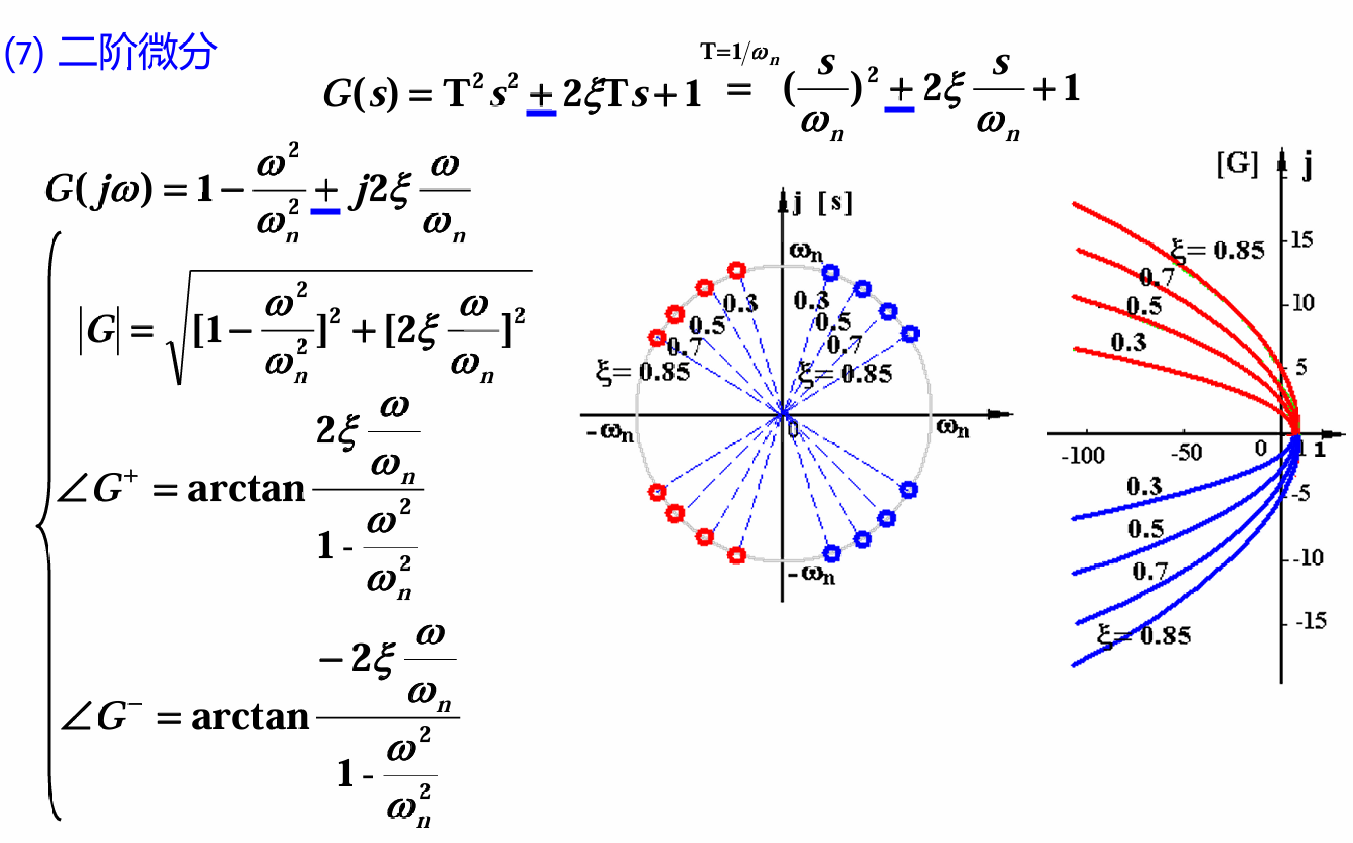
\includegraphics[width=.5\textwidth]{note/frequency-domain analysis/figure/4.png}\\
    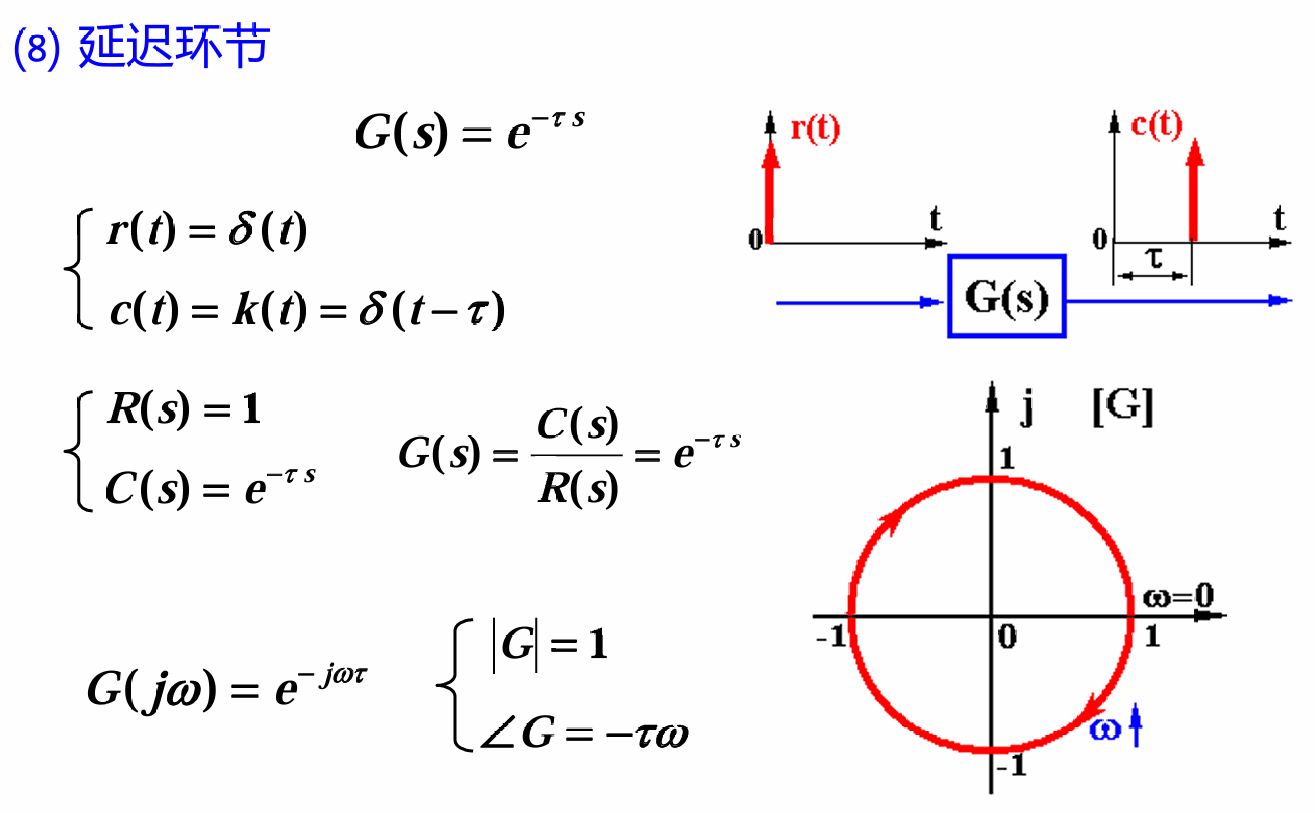
\includegraphics[width=.5\textwidth]{note/frequency-domain analysis/figure/5.png}\\
\end{center}

一般频率特性的Nyquist图绘制法如下：
\begin{enumerate}
    \item 当$\omega = 0$时，比例环节、惯性环节、振荡环节、一阶和二阶微分环节的幅角均为0°，只有积分环节当$\omega = 0^+$时幅角为-90°，所以当系统的开环传递函数中含有$v$个串联积分环节时，开环频率特性的Nyquist图在$\omega = 0^+$的起始处幅角为$v\cdot(-90\text{°})$
    \item 当$\omega = 0$时，比例环节的幅值为$K$，积分环节在$\omega = 0^+$时的幅值为$\infty$，其余各环节的幅值均为1，所以，开环幅频特性的幅值为：无积分环节$\omega = 0$时的幅值为$K$；有积分环节$\omega = 0^+$时幅值为$\infty$
    \item 当$\omega \to +\infty$时，开环频率特性Nyquist图中曲线的切线方向是$(n-m)\cdot(-90\text{°})$，其中m是分子的阶次，n是分母的阶次
    \item 当$\omega\to +\infty$时，开环频率特性Nyquist图沿$(n-m)\cdot(-90\text{°})$的方向趋向原点
\end{enumerate}
注意：
\begin{enumerate}
    \item 一个特殊点：谐振点：频率特性的幅值达到峰值的点（一般只有振荡环节存在），计算式如下：
    \begin{equation*}
        \omega_r = \omega_n\sqrt{1-2\zeta^2}
    \end{equation*}
    此时的峰值为：
    \begin{equation*}
        M_r = \left\lvert G(j\omega_r) \right\rvert =\frac{1}{2\zeta\sqrt{1-\zeta^2}}
    \end{equation*}
    \item 对于度数所对应的方向为：0°朝左，90°朝上，180°朝右，270°朝下
    \item 实际绘图时先把系统的频率特性（幅频和相频）写出来，观察式子中是否有间断点再绘图
\end{enumerate}



\subsubsection{Bode图}

频率特性$G(j\omega)$中的幅频特性和相频特性都是$\omega$的函数，Bode图是按照以下规律绘制的：
\begin{enumerate}
    \item 把幅频特性和相频特性分开画，横坐标为角频率$\omega$，纵坐标分别是频率特性的幅值和相角，画成两个曲线
    \item 在画频率特性时，角频率$\omega$的变化范围很大，几乎为$0\to +\infty$，所以将横坐标以10为底$\omega$的对数为长度划分，定义横坐标上每10倍频程之间的距离为一个单位长度，称作十倍频程（dec）
    \item 在Bode图的幅频特性中，纵坐标使用$L(\omega)$：
    \begin{equation*}
        L(\omega) = 20 \lg \left\lvert G(j\omega) \right\rvert 
    \end{equation*}

    此时即可将相乘转化为相加
    \item 在Bode图中，相频特性曲线的纵坐标时相频特性的角度本身$\angle G(j\omega)$，一般用°为单位，也可用弧度为单位
\end{enumerate}

典型环节的Bode图绘制如下所示：
\begin{center}
    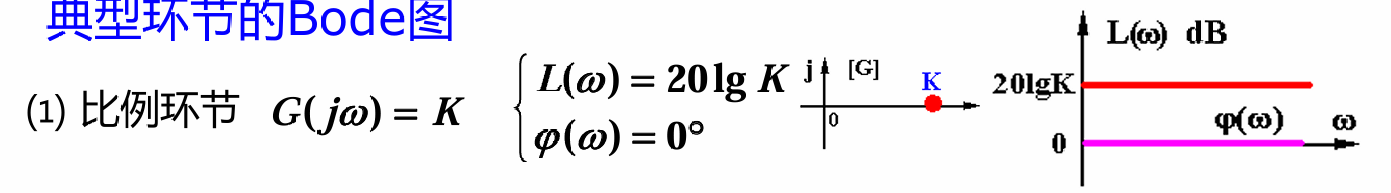
\includegraphics[width = .5\textwidth]{note/frequency-domain analysis/figure/6.png}\\
    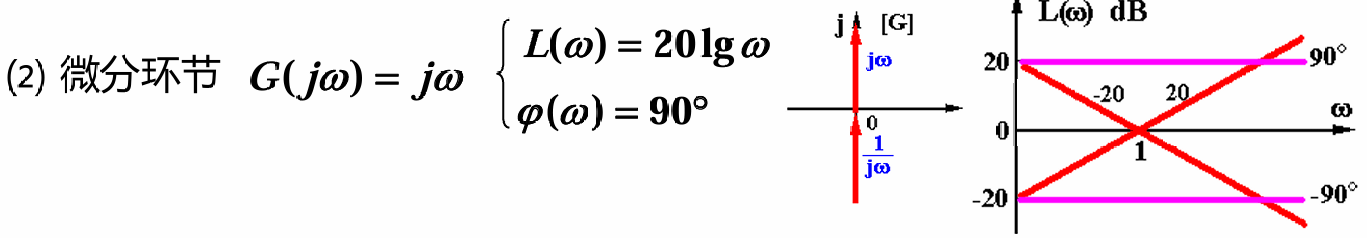
\includegraphics[width = .5\textwidth]{note/frequency-domain analysis/figure/7.png}\\
    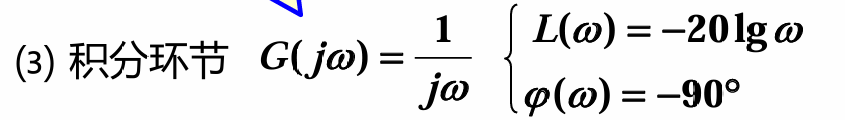
\includegraphics[width = .5\textwidth]{note/frequency-domain analysis/figure/8.png}\\
    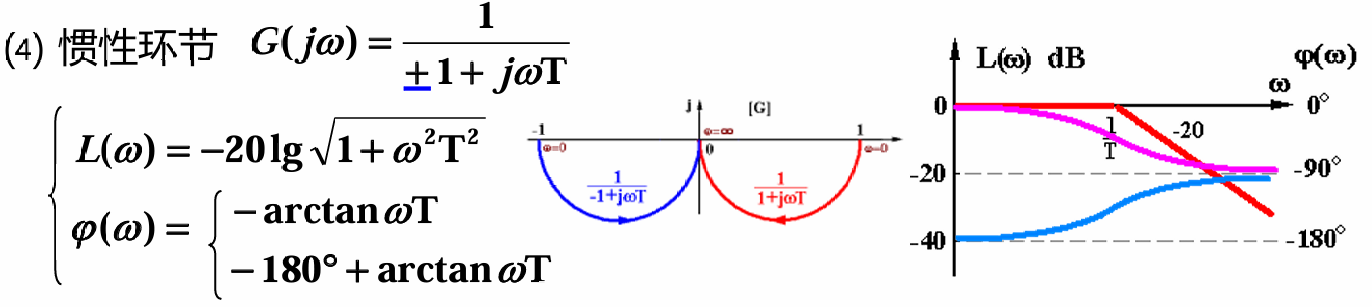
\includegraphics[width = .5\textwidth]{note/frequency-domain analysis/figure/9.png}\\
    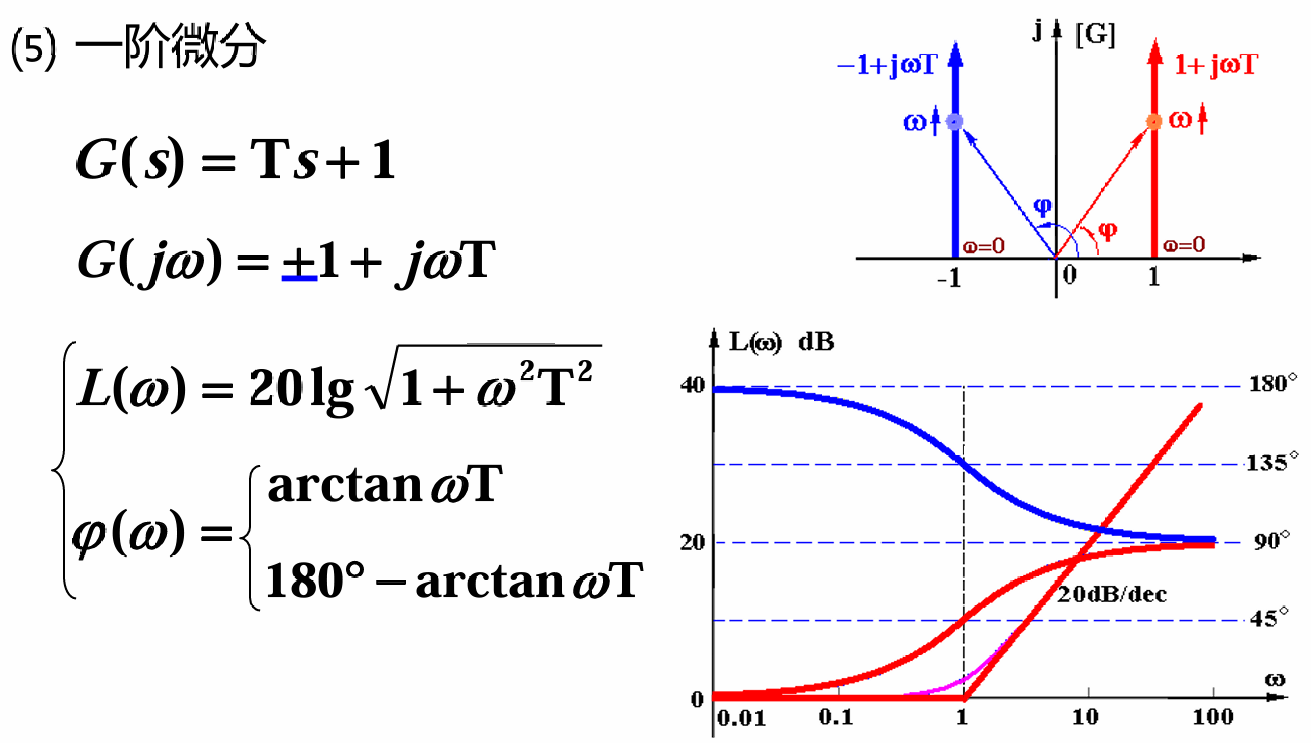
\includegraphics[width = .5\textwidth]{note/frequency-domain analysis/figure/10.png}\\
    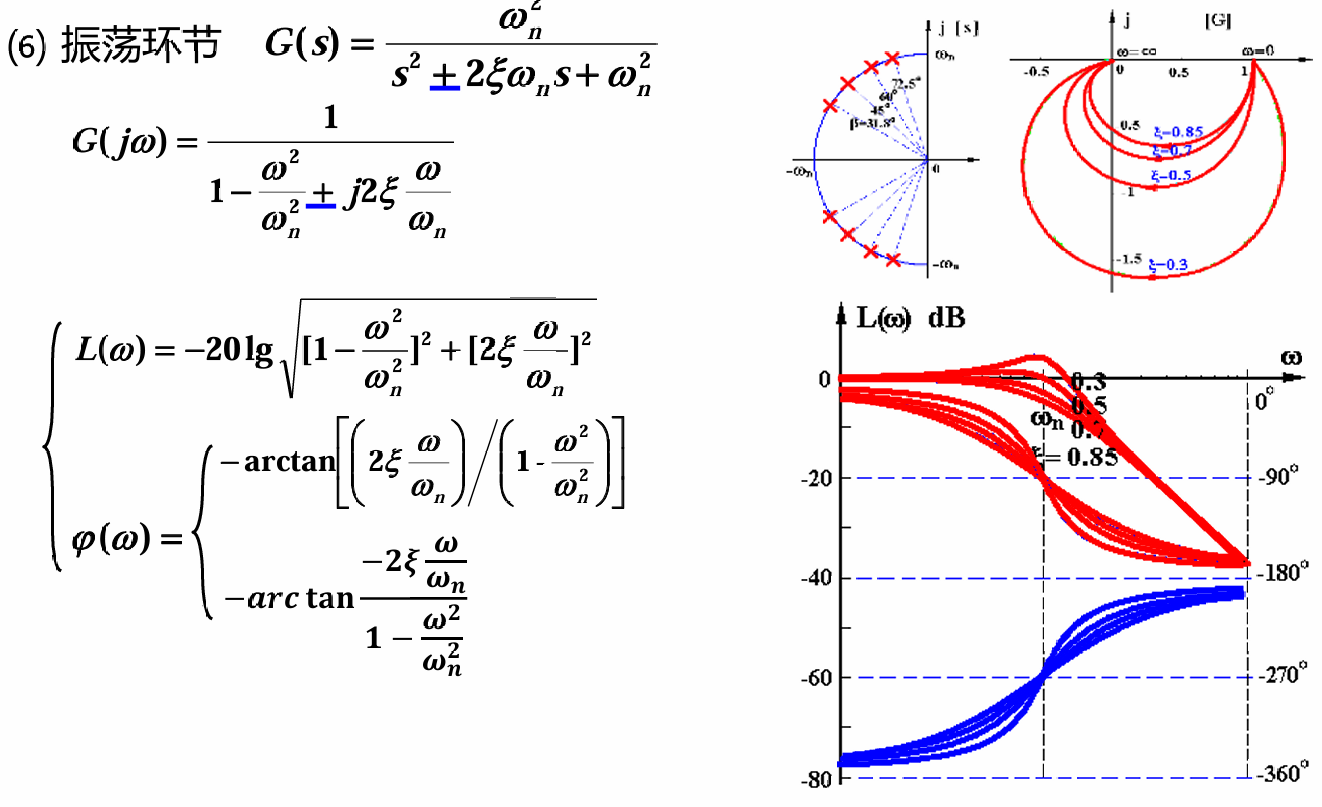
\includegraphics[width = .5\textwidth]{note/frequency-domain analysis/figure/11.png}\\
    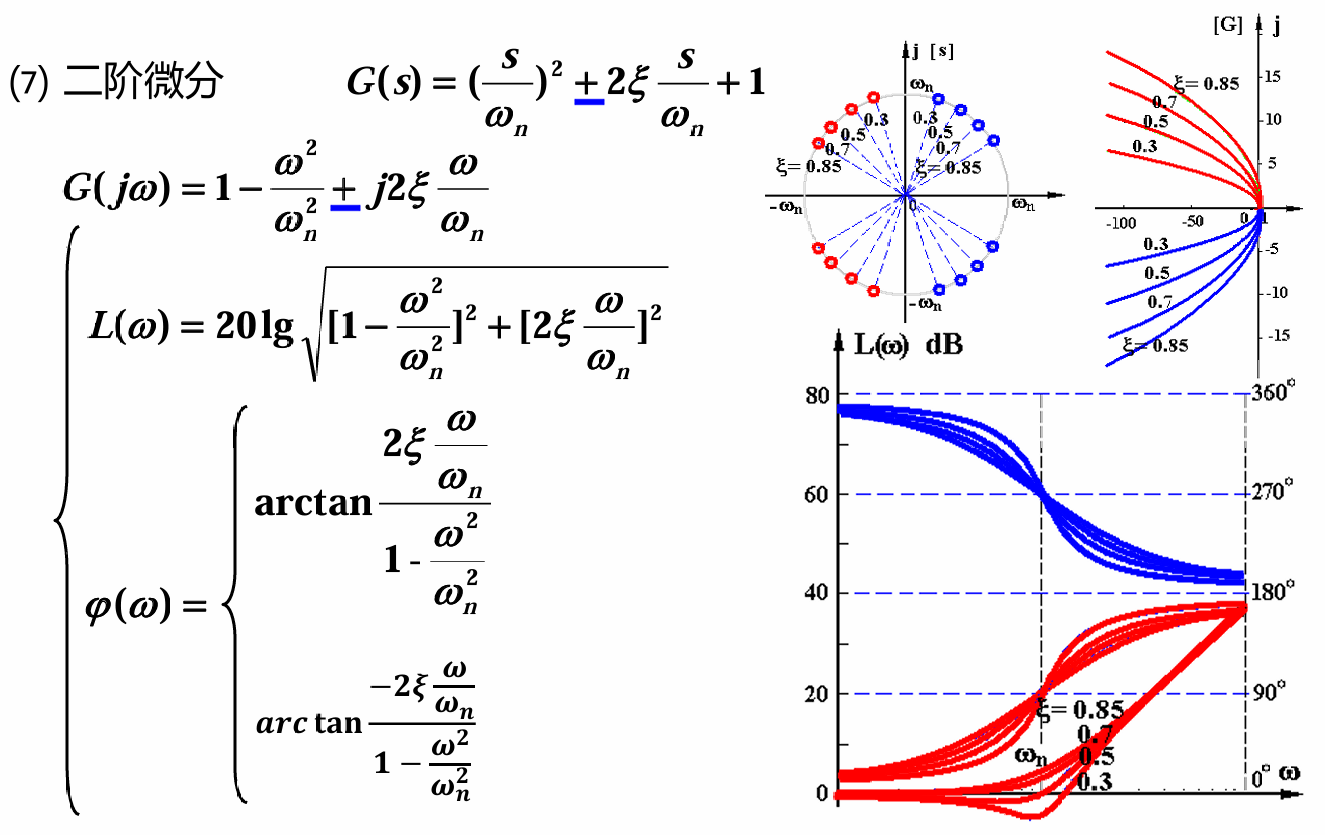
\includegraphics[width = .5\textwidth]{note/frequency-domain analysis/figure/12.png}\\
    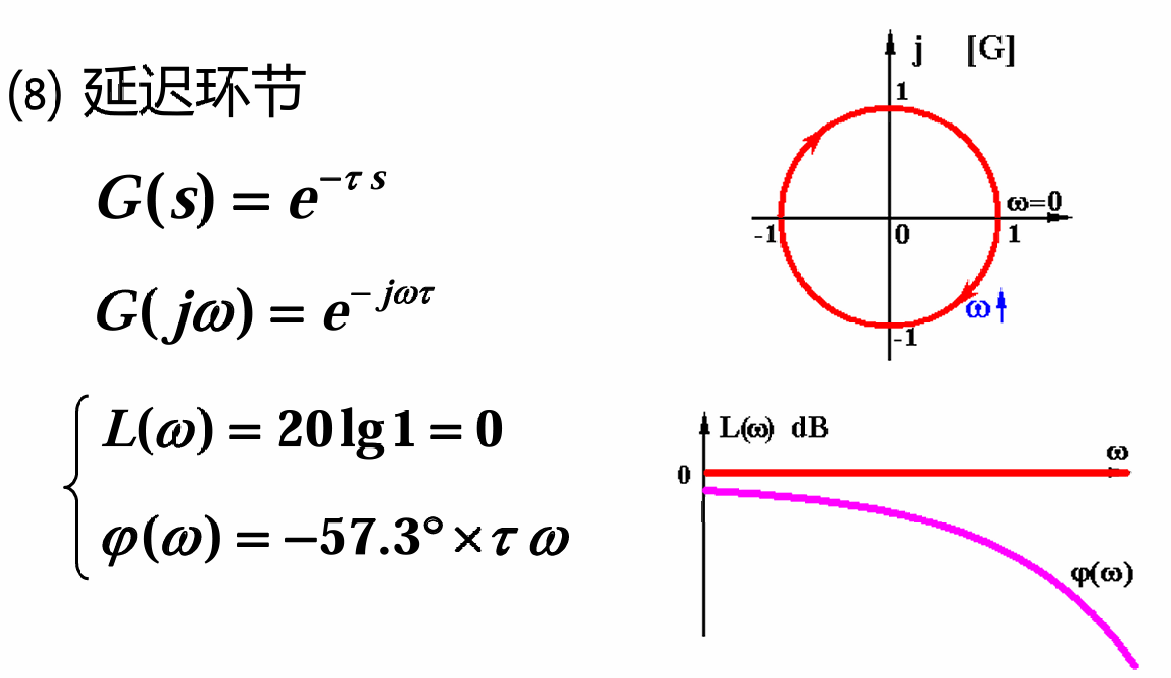
\includegraphics[width = .5\textwidth]{note/frequency-domain analysis/figure/13.png}
\end{center}

同样的，注意一个特殊点：剪切频率：Bode图中幅值特性第一次等于零的点，记为：$\omega_c$

\textbf{一般频率特性的Bode图的绘制}：

对数幅频特性与对数相频特性分别是各个串联环节的对数幅频特性之和与对数相频之和，所以只需做出各个环节的Bode图后将对应的幅频特性曲线与各个相频特性曲线相加即可，具体如下：
\begin{enumerate}
    \item 将$G(s)$化为频率特性标准型
    \item 按照顺序列出各个串联环节的转折频率（简化Bode图中斜率变化的点）
    \item 确定基准线（最小转折频率之左的特性及其延长线），此线过（1，$20\lg K$）
    \item 叠加作图（一阶$\pm 20$，二阶$\pm 40$）
    \item 在以下情况下修正简化Bode图：
    \begin{enumerate}
        \item 两惯性环节转折频率很接近时
        \item 振荡环节或二阶微分环节，此处有两种修正方式：
        \begin{itemize}
            \item 转折频率处修正，此时幅值差值（实际值-拟合值or虚线值-实线值）=$20\lg(\dfrac{1}{2\zeta})$（振荡环节）or = $20\lg(2\zeta)$（二阶微分环节）
            \item 谐振频率处修正，此时峰值$M_r = \dfrac{1}{2\zeta\sqrt{1-\zeta^2}}$，谐振频率$\omega_r = \omega_n\sqrt{1-2\zeta^2}$，bode图中为实际值-拟合值的绝对值为$20\lg M_r$
        \end{itemize}
    \end{enumerate}
    \item 检查Bode图是否正确：
    \begin{enumerate}
        \item 幅值特性曲线最右端斜率=-20(n-m)dB/dec
        \item 转折点数=惯性环节数+一阶微分数+振荡环节数+二阶微分数
        \item 相频特性在无穷处大小$\phi(\omega)\to -90\text{°}(n-m)$
    \end{enumerate}
\end{enumerate}